% === Add these to your preamble ===% keeps floats within their section
% (optional) Make [H] the default for all figures:
% \makeatletter\def\fps@figure{H}\makeatother
% ===================================


\chapter{Experiments and Results}

\section{Experiment 1.1}

\paragraph{Protocol.}
\begin{enumerate}
  \item Run the CLD-building algorithm:
    \begin{enumerate}
      \item Generate $N$ variables.
      \item Generate pairwise links.
      \item Insert spurious annotations during the iterative process.
    \end{enumerate}
  \item When the CLD is complete, apply \emph{LLM-as-a-Judge} on each edge annotation.
  \item Count the number of correctly and falsely classified hallucinations.
\end{enumerate}

\noindent The ``ground truth'' is a Sonar-Pro–generated CLD (later versions will use validated CLDs from the literature). Spurious annotations are created by prompting Sonar-Pro.

\begin{figure}[H]
  \centering
  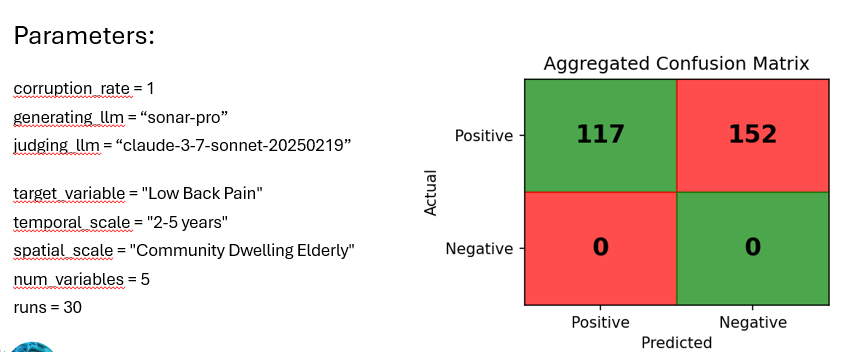
\includegraphics[width=0.5\linewidth]{exp-RQ1.1-llm-as-judge-corruptor-100.png}
  \caption{Experiment~1.1 with corruption rate $=1.0$ (run A).}
  \label{fig:rq1_1_100a}
\end{figure}

\begin{figure}[H]
  \centering
  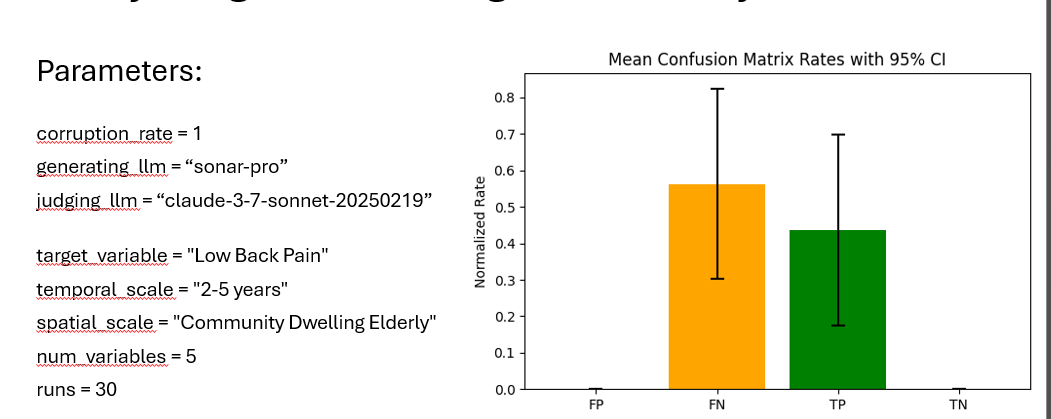
\includegraphics[width=0.5\linewidth]{exp-RQ1.1-llm-as-judge-corruptor-100b.png}
  \caption{Experiment~1.1 with corruption rate $=1.0$ (run B).}
  \label{fig:rq1_1_100b}
\end{figure}

\begin{figure}[H]
  \centering
  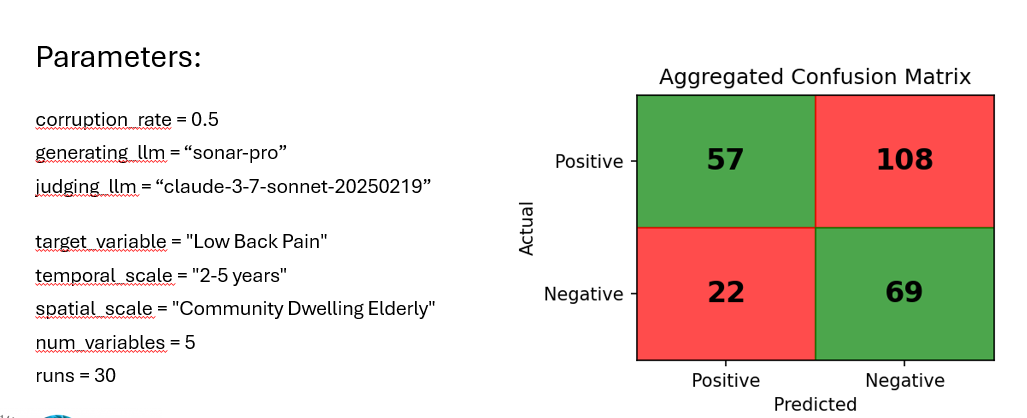
\includegraphics[width=0.5\linewidth]{exp-RQ1.1-llm-as-judge-corruptor-50a.png}
  \caption{Experiment~1.1 with corruption rate $=0.5$ (run A).}
  \label{fig:rq1_1_50a}
\end{figure}

\begin{figure}[H]
  \centering
  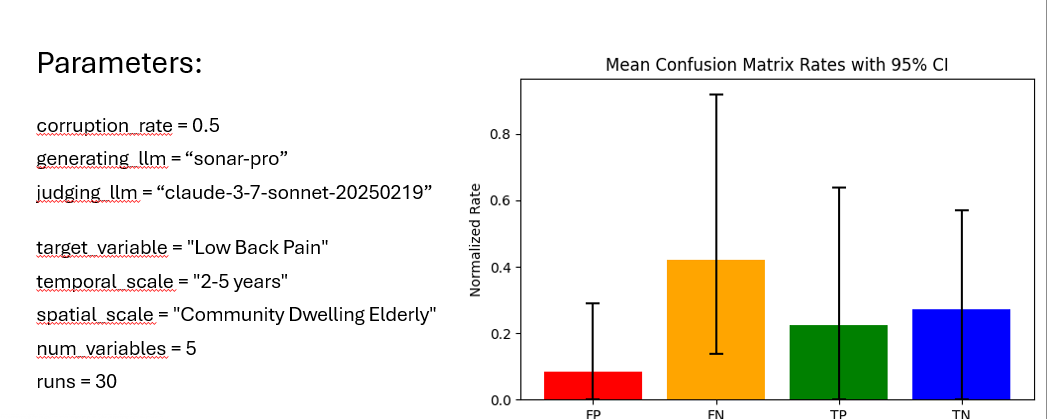
\includegraphics[width=0.5\linewidth]{exp-RQ1.1-llm-as-a-judge-corruptor-50b.png}
  \caption{Experiment~1.1 with corruption rate $=0.5$ (run B).}
  \label{fig:rq1_1_50b}
\end{figure}

\paragraph{Findings.}
\textbf{Experiment 1 (corruption rate $=1$).}
True positives indicate the Judge can detect spurious annotations; false negatives show the Judge is imperfect at detecting them.

\noindent\textbf{Experiment 2 (corruption rate $=0.5$).}
The Judge makes more errors in a semi-spurious mixed dataset; both false negatives and false positives increase. Large CIs indicate inconsistency in performance. At least TP~$>$~FP on average, but the non-overlapping CIs suggest this may not be significant.\footnote{Note: the ``ground truth'' may be flawed.}

\section{Experiment 1.1c: parallel ensemble judging}

\begin{figure}[H]
  \centering
  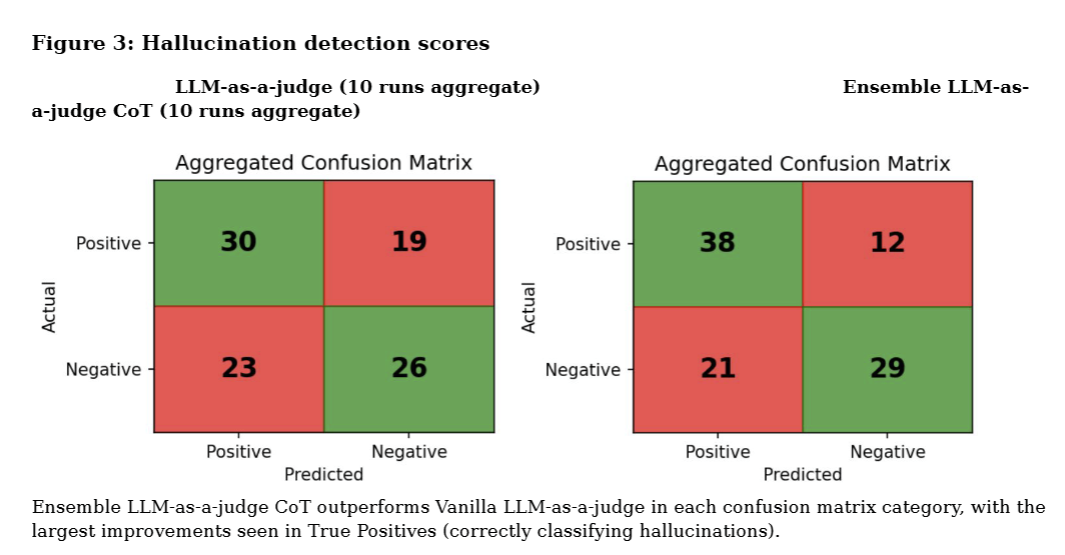
\includegraphics[width=0.5\linewidth]{exp-RQ1.1c-parralel-judging-conf-matrices.png}
  \caption{Confusion matrices for parallel ensemble judging (Experiment~1.1c).}
  \label{fig:rq1_1c_conf}
\end{figure}

\begin{figure}[H]
  \centering
  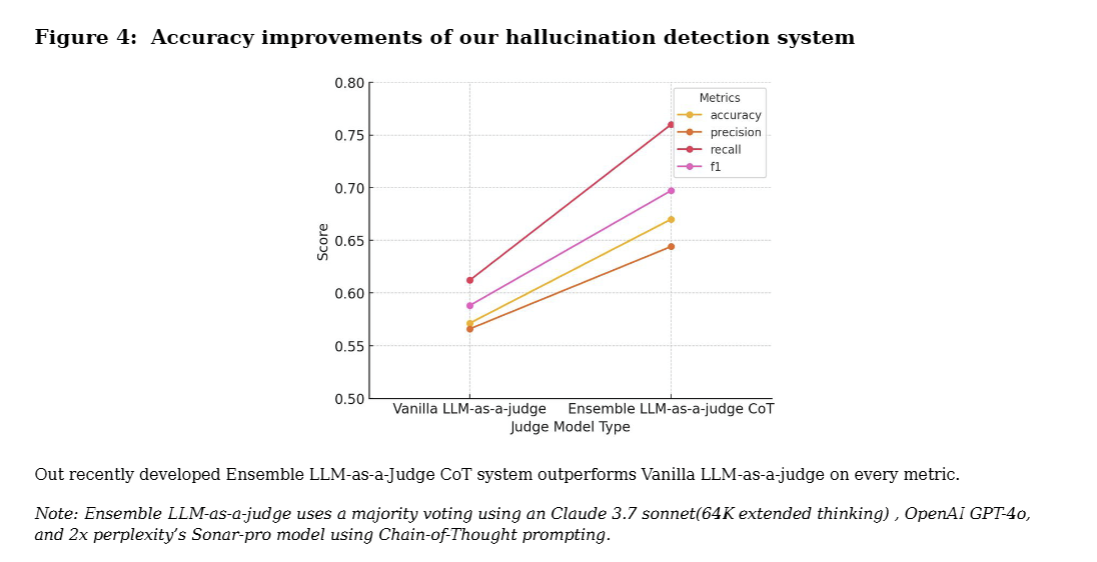
\includegraphics[width=0.5\linewidth]{exp-RQ1.1c-parralel-judging-comparison-linear-plot.png}
  \caption{Comparison plot for parallel ensemble judging (Experiment~1.1c).}
  \label{fig:rq1_1c_comp}
\end{figure}

\begin{figure}[H]
  \centering
  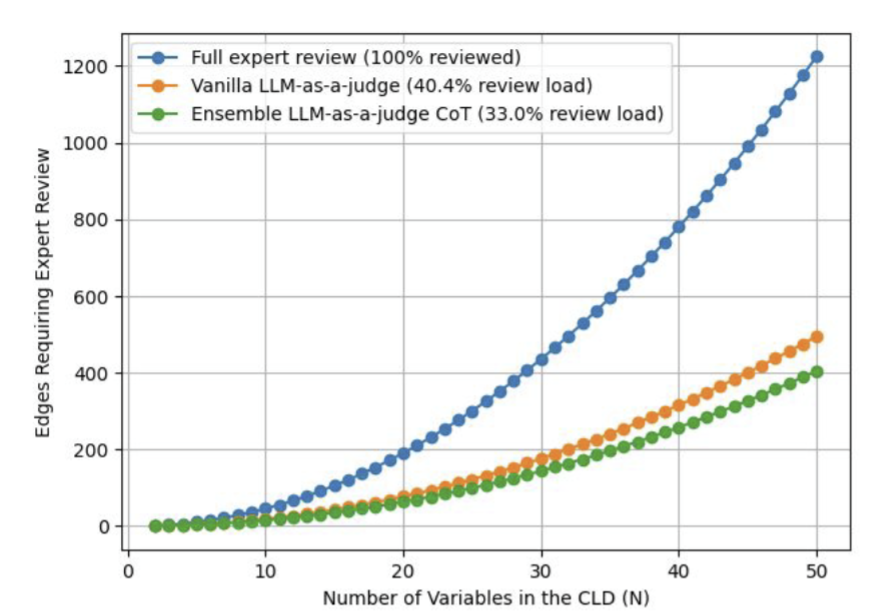
\includegraphics[width=0.5\linewidth]{exp-RQ1.1-impact-cost-saving-by-hallucination-reduciton.png}
  \caption{Estimated impact and cost savings from hallucination reduction.}
  \label{fig:rq1_cost_saving}
\end{figure}

\section{Cost scaling}

\begin{figure}[H]
  \centering
  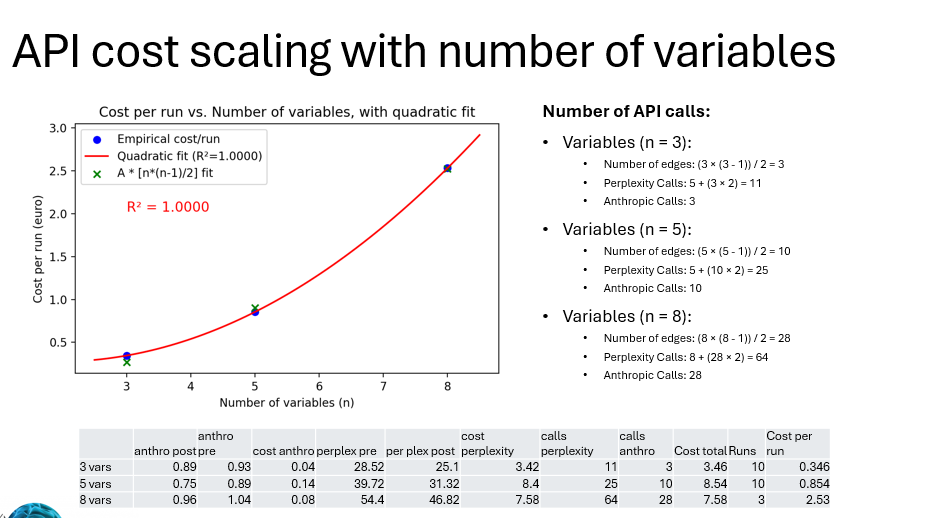
\includegraphics[width=0.5\linewidth]{exp-RQ3.prelim-cost-scaling-with-N.png}
  \caption{Preliminary cost scaling with $N$.}
  \label{fig:rq3_cost_scaling}
\end{figure}

\section{Parameter experiments}

\begin{figure}[H]
  \centering
  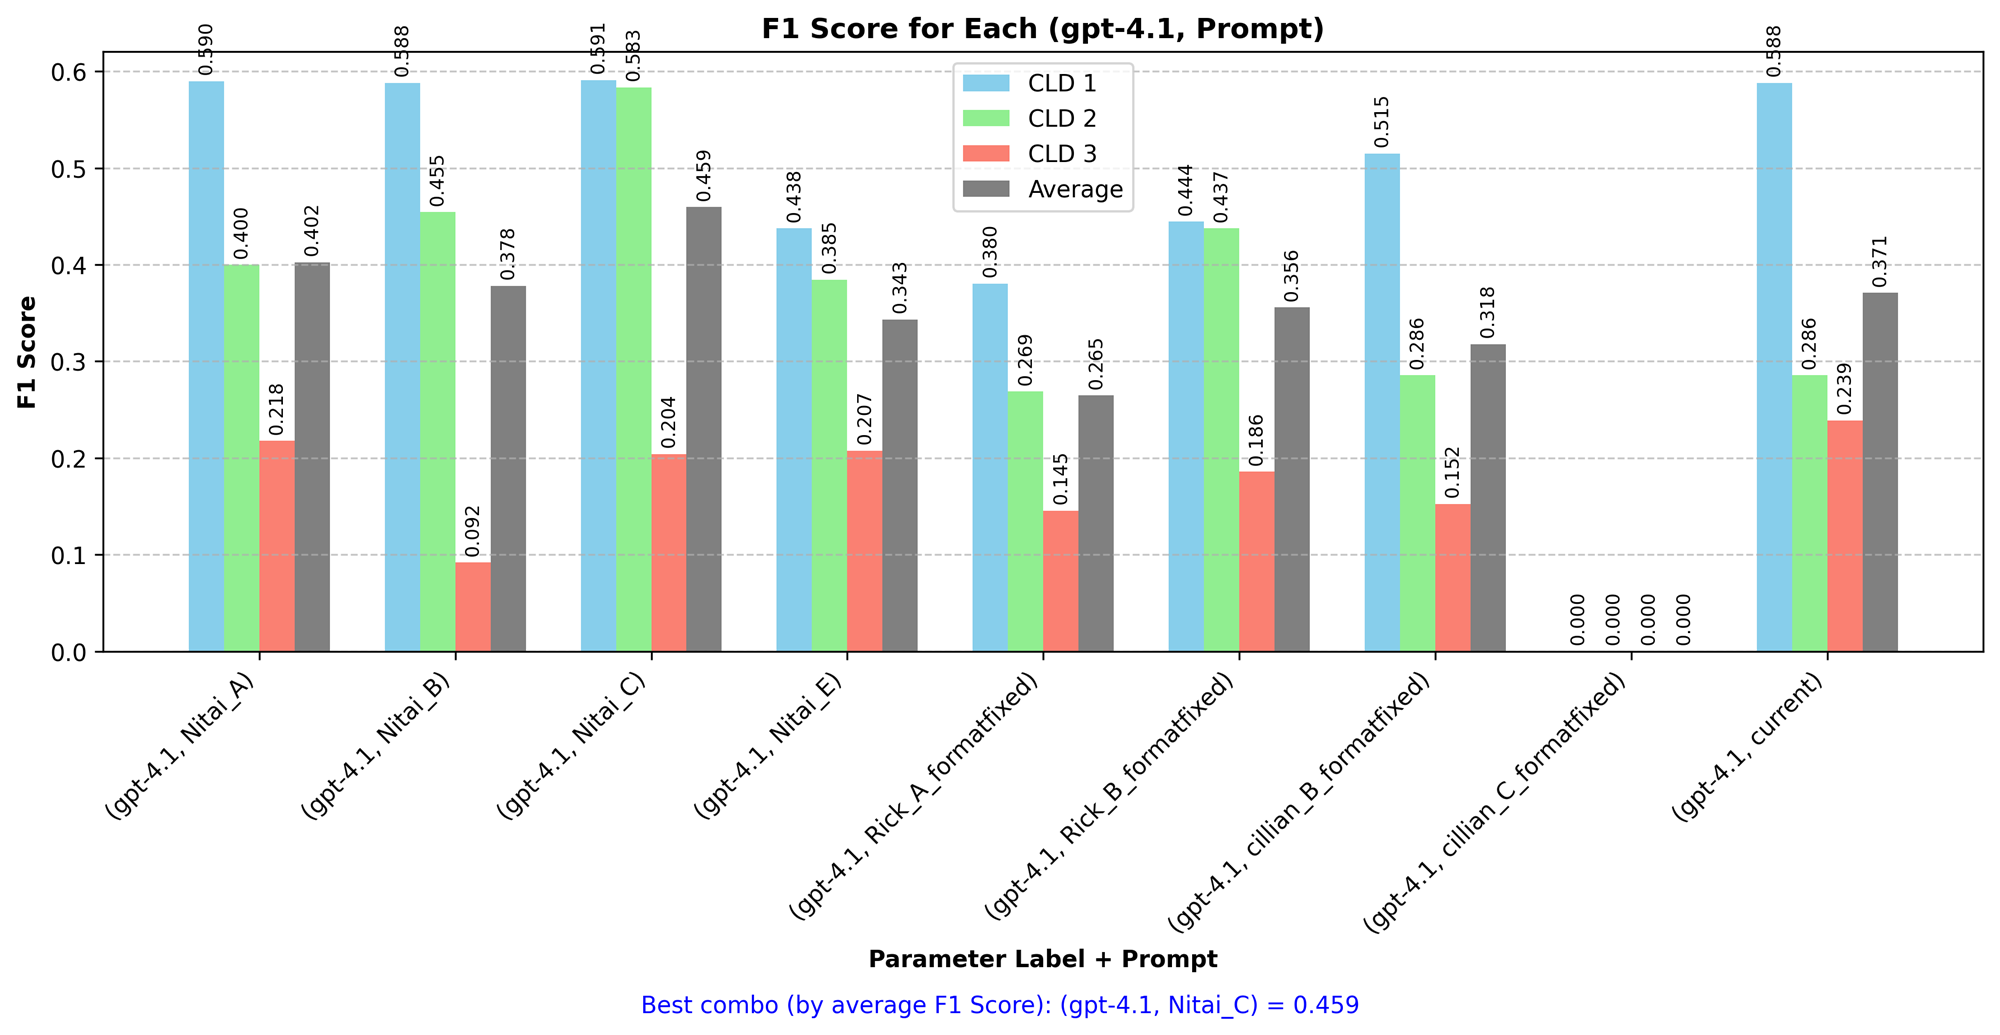
\includegraphics[width=0.5\linewidth]{exp-param-prompt-model-vs-3CLD-ground-truth.png}
  \caption{Model/prompt comparison against 3-CLD ground truth.}
  \label{fig:param_prompt_vs_gt}
\end{figure}

\section{Cost scaling with variable $N$}

\begin{figure}[H]
  \centering
  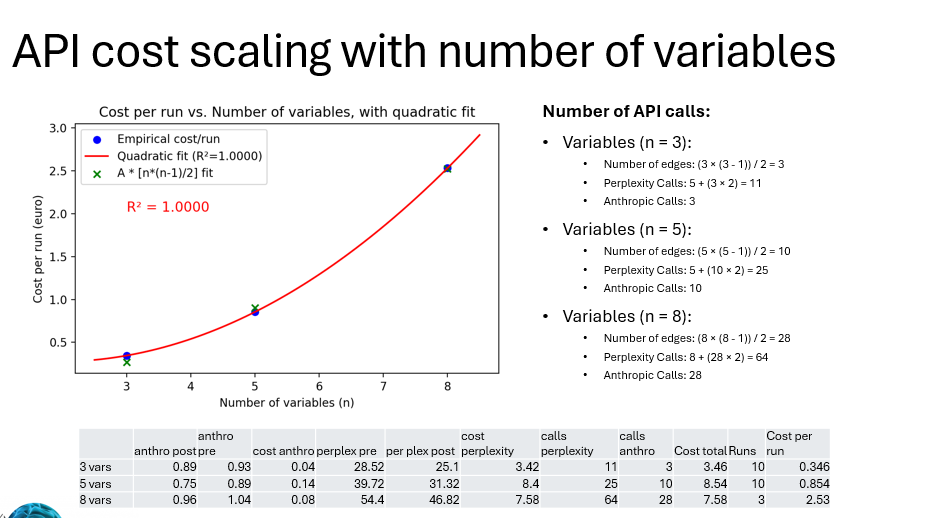
\includegraphics[width=0.5\linewidth]{exp-RQ3.prelim-cost-scaling-with-N.png}
  \caption{Cost scaling as a function of variable $N$.}
  \label{fig:rq3_cost_scaling_varN}
\end{figure}


\section{Temperature scaling}

\begin{figure}
    \centering
    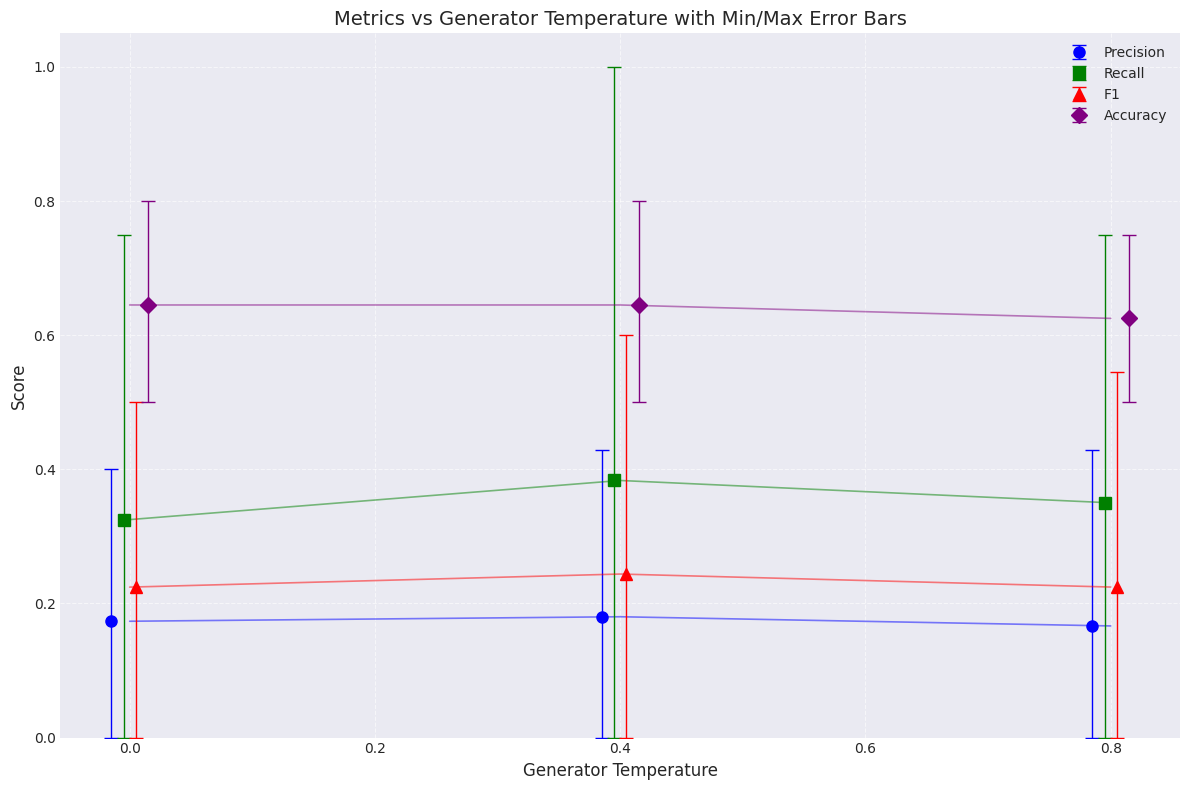
\includegraphics[width=0.5\linewidth]{exp-param-temperature-summary-f1-arracy-recall-recision-as-function-of.png}
    \caption{Enter Caption}
    \label{fig:placeholder}
\end{figure}


\begin{figure}
    \centering
    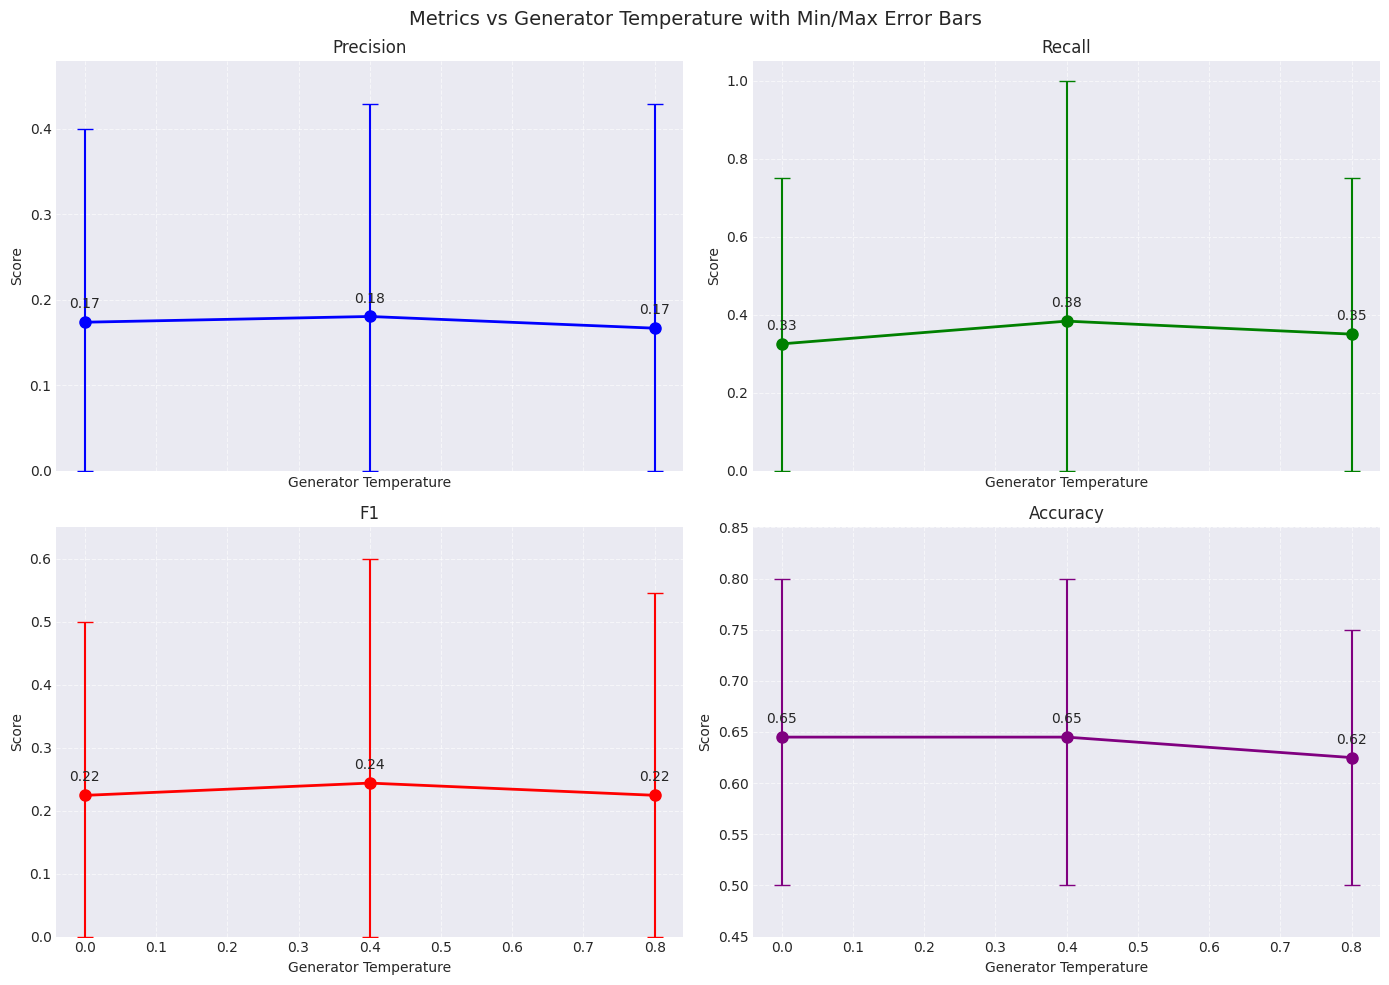
\includegraphics[width=0.5\linewidth]{exp-param-temperature-f1-arracy-recall-recision-as-function-of-temperature.png}
    \caption{Enter Caption}
    \label{fig:placeholder}
\end{figure}


\begin{figure}
    \centering
    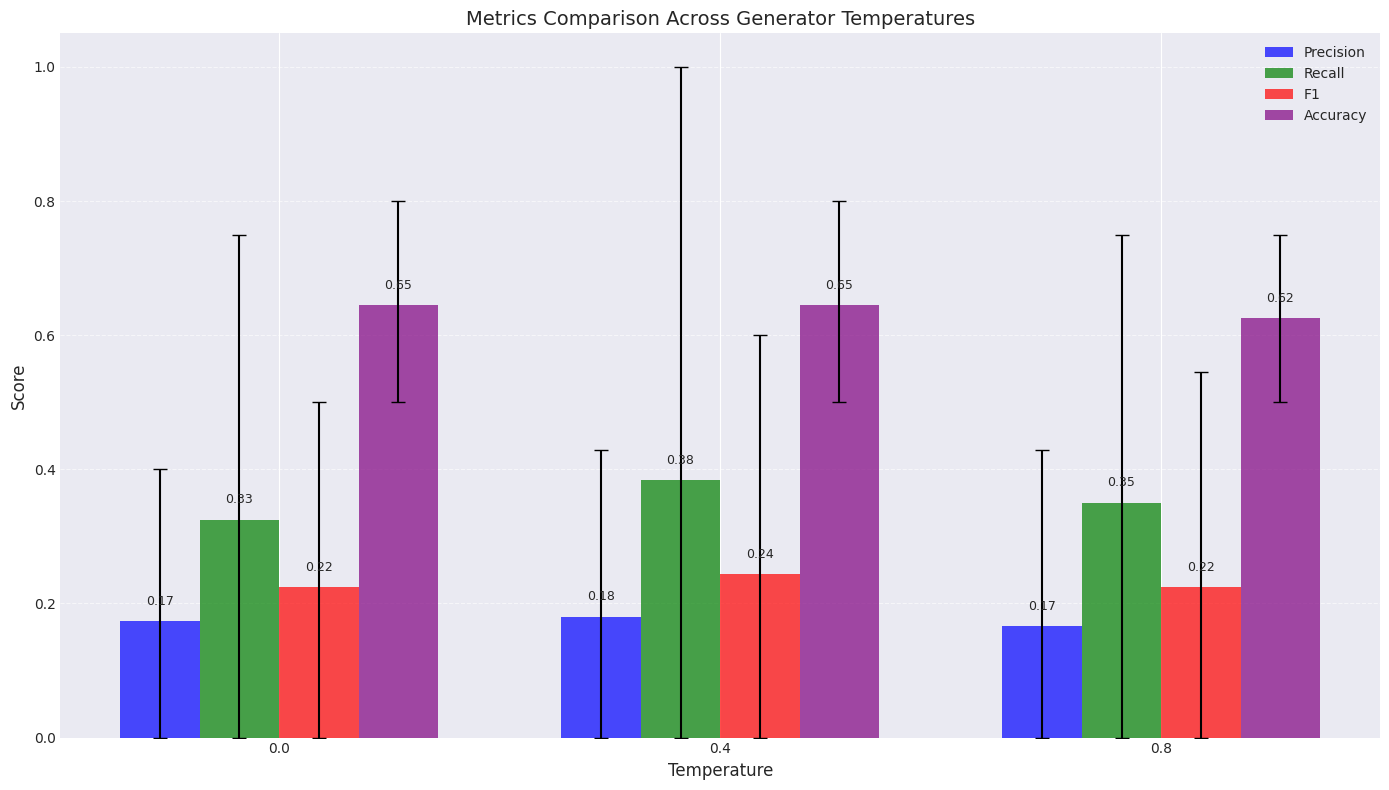
\includegraphics[width=0.5\linewidth]{exp-param-temperature-barchat-f1-arracy-recall-recision-as-function-of.png}
    \caption{Enter Caption}
    \label{fig:placeholder}
\end{figure}


